\documentclass{article}
\usepackage{graphicx} % Required for inserting images
\usepackage{multicol}
\usepackage{amsthm}
\usepackage{amsmath}
\usepackage{amssymb}
\usepackage{xcolor}
\usepackage{mathtools}
\usepackage{centernot}

\DeclarePairedDelimiter\ceil{\lceil}{\rceil}
\DeclarePairedDelimiter\floor{\lfloor}{\rfloor}

\title{AICC II}
\author{Simon Lefort Laura Paraboschi}
\date{February 2024}

\newtheorem{definition}{Definition}[section]

\begin{document}

\maketitle

\section{Entropy and Data Compression}

\subsection{Sources and Entropy}

Let $ S $ be a \textbf{random variable}, a function that associates a \textbf{real number} to each \textbf{outcome}, $ s $.

\begin{quote}
    For example, a random variable can be X, that counts the number of $ 6 $ after 2 throws.
    \begin{equation}
        H(s) =
        \begin{cases}
            0 & \text{if $ s $ is "we got no 6"}\\
            1 & \text{if $ s $ is "we got a single 6"}\\
            2 & \text{if $ s $ is "we got two 6"}
        \end{cases}
    \end{equation}
\end{quote}
Let $ A $ be \textbf{the alphabet} for this symbol (all the possible outcomes). Therefore, there are $ |A|^n $ possible values for $ n $ successive symbols.
\paragraph{Support} The support of a random variable is all the outcomes $ s $ such that $ p(S = s) \equiv p_S(s) > 0 $.

\paragraph{Entropy} The entropy of a random variable represents the level of "uncertainty", "surprise" related to the variable's possible outcomes. 
\[ H_b(S) := - \sum_{S \in A} p_S(s)log_b(p_S(s))\]
In this course, $ b $ will almost always be $ 2 $, because we are interested in binary representation of data. 
\begin{quote}
    Note that we can also compute the expected value of $ -log(p_S(S)) $.
    \begin{equation} \label{eq1}
        \begin{split}
            H(S) & = \mathbb{E}[-log_b(p_S(S))] \\
            & = \sum_{s \in A} p_S(s) \cdot -log_b(p_S(s))
        \end{split}
    \end{equation}
\end{quote}
\paragraph{Uniform distribution} We say that a random variable is uniformly distributed if:
\[ \forall s \in A, p(s) = \frac{1}{|A|}\]
In that case the entropy of $ A $ is the maximum, $ log(|A|) $.\\
Indeed:
\[ 0 \text{ (no randomness) } \leq H_b(S) \leq log_b|A| \text{ (max randomness) } \]

\begin{figure}
    \centering
    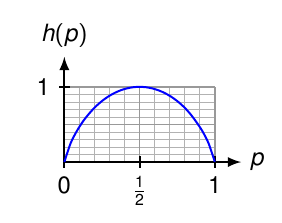
\includegraphics[width=0.4\linewidth]{entropy.png}
    \caption{when $|A| = 2, h(p_s(s)) $ is entropy}
    \label{fig:enter-label}
\end{figure}

\paragraph{IT-Inequality} (useful for demos) the \textbf{IT-inequality} states that:
\[ log_b(r) \leq (r-1)log_b(e) \]
with equality iff $ r = 1 $.

\paragraph{Sequence of random variables} A sequence of random variable is finite $ (S1,...,S_n) $ or infinite $ S_1, S_2, ... $. The probability that the sequence happens is denoted by $ p_{S_1,...S_n}) $. We can then compute the entropy $ H(S_1,...,Sn_) $.\\
\textbf{Note:}
\[ H(S_1,S_2,...,S_n) \leq H(S_1) + ... H(S_n) \]
with equality iff $ S_1,...,S_n $ are independent. Seems "intuitive" because there is less "surprise" if you know one outcome is "linked" to another one.

\paragraph{Marginal distribution}, or $ p_X(x) $, can be calculated by summing over all the outcomes of $ Y $ the value of $ p_{X,Y}(x/y) $.

\paragraph{Joint distribution}, often represented as a table, gives us the probability that $ X = x $ and $ Y = y $.

\subsection{Source Coding}

\paragraph{Encoder} An encoder is defined by:
\begin{itemize}
    \item the input alphabet $ \mathbf{A} $
    \item the output alphabet $ \mathbf{D} $ (typically $ {0,1} $)
    \item the codebook $ \mathbf{C} $ which consists in sequences of $ D $
    \item a one-to-one function $ \Gamma : \mathbf{A}^k \to \mathbf{C} $
\end{itemize}

\paragraph{Prefix-free codes} are codes where no cdeword is the prefix of another word.

\paragraph{Unique decodability} is verified if every concatenation of codewords can a unique parsing into a sequence of codewords (\textit{can you decode with only one solution?})

\begin{itemize}
    \item fixed-length code $ \implies $ uniquely decodable
    \item prefix-free $ \implies $ uniquely decodable
    \item prefix-free $ \equiv $ instantaneous
    \item reverse is prefix-free $ \neg \implies $ instantaneous
\end{itemize}

\paragraph{Kraft-McMillan theorem} Let $ I_1, ..., I_m $ be the respective codewords lengths.\\
\[ \text{D-ary code uniquely decodable} \implies D^{-I_1} + ... + D^{-I_m} \leq 1 \]
(intuition: comes from the number of used leaves)

\paragraph{Kraft-McMillan theorem 2} if the positive integers $ I_1, ..., I_m $ satisfy the Kraft's inequality for some integer $ D $, there exists a D-ary prefix-free code.\\
To build it, draw a tree and order codewords lengths in increasing order.

\paragraph{Average codeword length} takes into account the probability a character appears.
\[ L(S, \Gamma) := \mathbf{E}[l(S)] = l_a \cdot p(S = a) +l_b \cdot p(S = b) + ... + l_z \cdot p(S = z) \]
\[ \mathbf{\Leftrightarrow L(S, \Gamma) = \sum_{s \in A} p_s(s) \cdot l(\Gamma(s))} \]
Unit for codeword length is "code symbols" (or bits in most cases in this class).

\paragraph{Shannon codes} are prefix-free codes where the length of each symbol is calculated this way:
\[ l(\Gamma(s)) = \ceil*{-log_D(p_S(s))} \]
These are clearly \textbf{not optimal} codes (but they are still uniquely decodable and easy to create). Also, the following identity applies:
\[ H_D(S) \leq L(S, \Gamma_{Shannon}) < H_D(S) + 1 \]
\begin{quote}
proof lower bound: $ H_D(S) - L(S, \Gamma) \leq 0 $ (+ IT ineq.)\\
proof upper bound: as we use $ \ceil*{-log_D(p_S(s))} < -log_D(p_S(s)) + 1$
\end{quote}

\paragraph{Huffman codes} construction, unlike Shannon codes, start from the leaves. We write the probability of each symbol, and recursively join the ones with the smallest probability. Such codes are \textbf{optimal} (the best we can have). They are not necessarily unique.

\begin{figure}[h]
    \centering
    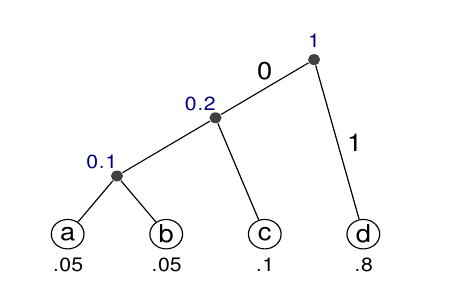
\includegraphics[width=0.5\linewidth]{huffman.png}
    \caption{0.05/0.05 then 0.1/0.1 then 0.2/0.8}
    \label{fig:enter-label}
\end{figure}

When using D-ary code, at the beginning, we need $ k(D-1) + D $ leaves.

\paragraph{Path-Length lemma} states that you can compute the average length of a code by simply summing over the probabilities of the intermediate nodes \textit{(here, 0.1 + 0.2 + 1 = 1.3)}.

\newpage

\paragraph{Compressing long strings}, concatening Huffman codes $ n $ times no longer produce the best result. We need to make a new Huffman codes for \textbf{blocks} of $ n $ letters and associated probabilities. The per letter average codeword-length bcomes (in a 2-letter example):
\[ \frac{H_D(S_1, S_2)}{2} \leq \frac{L((S_1, S_2), \Gamma_{SF})}{2} < \frac{H_D(S_1, S_2)}{2}  + 1 \]
for $ S_1, S_2, ..., S_n $ (dependent OR independent):
\[ \frac{H_D((S_1, S_2, ..., S_n)}{n} \leq \frac{L((S_1, S_2, ..., S_n), \Gamma_{SF})}{n} < \frac{H_D((S_1, S_2, ..., S_n) + 1}{n} \]
or, if $ S_1, S_2, ..., S_n $ are independent and identically distrib. (IID):
\[ H_D(S) \leq \frac{L((S_1, S_2, ..., S_n), \Gamma_{SF})}{n} < H_D(S) + \frac{1}{n} \]
(because $ H(S_1) = H(S_2) = ... = H(S_n) = nH(S)) $\\\\
Therefore when compressing long strings, \textit{"it's no longer entropy and entropy +1, entropy is it"} - Gastpar

\paragraph{IID Source} from now on we will think about sources, that emits an (possibly) infinite sequence of symbols. IID sources are \textbf{independent} from each other and \textbf{identitcally distributed} according to a fixed distribution $ p_S(s) $ (not really the case in the real world).\\\\Thus : let $ S $ be the infinite sequence produced by an IID source $ S $.
\begin{itemize}
    \item by encoding blocks of symbols into D-ary codewords, the average codeword-length per symbol of a uniquely decodable code can be made as close as desired to $ H_D(S) $
    \item no uniquely decodable D-ary code can achieve a smaller average codeword-length
\end{itemize}
\[ H(S_{\text{IID source}}) = log(|\text{IID source}|) \]

\newpage

\subsection{Conditional Entropy}

In real world sequences, strings are not i.i.d.
 
\paragraph{Conditional probability} gives the probability of the event $ X = x $ given that $ Y = y $ has occured
\[ p_{X/Y}(x/y) = \frac{p_{X,Y}(x, y)}{p_Y(y)}\]

\paragraph{Average conditional entropy} is the average entropy of a variable $ X $ knowing $ Y $ (but not knowing exactly what little $ y $ is).
\[ H(X/Y) = \sum_{y \in Y} p(Y = y) (\sum_{x \in X} p(x/y)\cdot{\log_{D}(p(x/y))} \leq H(X) \]
\[ \Leftrightarrow \sum_{y \in Y} H(X/ Y = y)p(Y = y) \]
with equality iff X, Y are independent:
\[ \text{X, Y independent} \Leftrightarrow H(X/Y) = H(X) \Leftrightarrow p(x, y) = p(x)p(y) \]

\paragraph{Conditional entropy bound} can we say that \textbf{with a fixed little y}:
\[ H_D(X/Y = y) \leq_{?} H_D(X) \]
It would seem intuitive, but no!
\begin{quote}
    \begin{itemize}
        \item Let X : 1 if I follow the lecture, 0 otherwise
        \item I come to the campus $ 99\% $ of the time
        \item I follow the lecture $ 100\% $ of the time if I come to the campus
        \item I follow the lecture $ 50\% $ of the time if I do not come to the campus
        \item Let Y : 1 if my car is broken, 0 otherwise
        \item The entropy of X is lower than the entropy of X knowing Y = 1.
    \end{itemize}
\end{quote}

\paragraph{Conditional entropy of f(x)}, where f is a deterministic function
\[ H(f(x)/x) = 0 \]

\paragraph{Chain rule}
\[ H_D(X, Y) = H_D(X) + H_D(Y/X) \]
\[ \Leftrightarrow H_D(Y, X) = H_D(Y) + H_D(X/Y) \]
\[ \Leftrightarrow H(X/Y) = H(X, Y) - H(Y) \]
therefore:
\[ H_D(S_1, ..., S_n) = H_D(S_1) + H_D(S_2/S_1) + ... + H_D(S_n/S_1, ..., S_{n-1}) \]

\paragraph{Entropy rate} à quel point quand on ajoute une lettre à notre code ça fait descendre vers l'avg code length vers l'entropie ?

\paragraph{Sunny-Rain source} probability of next symbol only depends on the previous one

\begin{figure}[h]
    \centering
    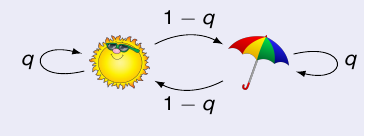
\includegraphics[width=0.75\linewidth]{sunnyrain.png}
    \caption{Enter Caption}
    \label{fig:enter-label}
\end{figure}

Compute probability of $ c $ swaps starting with a specific R or S.
\[ p_{s_1, s_2, ..., s_n}(s_1, ..., s_n) = \frac{1}{2} \cdot q^{n-1-c}(1-q)^c \]
$ (1-q) $ represents the swaps

\paragraph{Distribution of a random variable X} is now denoted as $ p_X(\cdot) $.

\paragraph{Regular source} $ \mathbb{S} = (S_1, S_2, ...) $ if:
\[ H(\mathbb{S}) = \lim_{n\to \infty} H(S_n) \]
\[ H^{*}(\mathbb{S}) \text{ (entropy rate) } = \lim_{n\to\infty} H(S_n|S_1,S_2,...,S_{n-1}) \]
exist and are finite.
\[ H^{*}(\mathbb{S}) \leq H(\mathbb{S}) \]
For regular sources:
\[ H^{*}(\mathbb{S}) = \lim_{n\to\infty} \frac{H(S_1,...,S_n)}{n} \]

\paragraph{Stationary source} if statistics, probabilities never change over time.

\paragraph{Known bounds on factorial}

\[ \frac{n^n}{e^{n-1}} \leq n! \leq \frac{n^{n+1}}{e^{n-1}} \]

\subsection{Entropy and algorithms}

\paragraph{Algorithmic performance} can be bounded using entropy (for example, we know we would need at least X questions before finding a word correctly, on average for the 20 questions game).

\newpage

\section{Cryptography}

\paragraph{Monoalphabeticalphabet cipher} is a unique bijection between a fixed alphabet and a new alphabet of the same size.

\paragraph{Polyalphabetic cipher} (like Vigenere) uses multiple substitution tables (a key specify which table is used for which position in the message).

\paragraph{Perfect secrecy}, when knowing the cryptogram does not give you any guess about the plaintext, they are statistically independent (where T is the plaintext, K is the key) and it implies:
\[ H(T) \leq H(K) \]

\paragraph{Symmetric-key cryptosystem} is one for which both ends use the same key (for encryption then decryption). Problem: in a n-user network, each user needs n-1 keys to communicate. It's very expensive to distribute securely keys.

\paragraph{One-way function} ex. $ g \to g^a \mod{p} $. For reverse, it's a discrete logarithm problem to compute a such that $ g^a \mod p = A $

\paragraph{Exchanging keys (Diffie and Hellman)} We agree on a $ p $ prime and a generator (see below).
Let $ a $ the secret known by A, and $ b $ the secret known by  B $ \in \{ 1, 2, 3, ..., t-1 \} $
\begin{itemize}
    \item $ g^a $ is sent to B
    \item $ g^b $ is sent to A
\end{itemize}
therefore, the attacker knows $ g^a, g^b $ but can not compute $ g^{ab} $ while A and B can.

\paragraph{Exchanging plaintext} same as before, but now A sends :
\begin{itemize}
    \item $ g^a $
    \item $ t \cdot {g^{ab} \mod p} $
\end{itemize}
B needs to compute $ C $ s.t. $ C \cdot g^{ab} \mod p = 1 $.
So then B can can $ t = C \cdot g^{ab} \cdot t \mod p $

\newpage

\subsection{Number theory}

\paragraph{Euclidian division}, $ a = m \cdot q + r $, $ r $ has to be positive $ \in \{0,1,2,3,4,5,...,m-1\}$
if $ a \mod m $ is non negative, then $ r = a \mod m $, otherwise $ r = a \mod m + m $

\paragraph{Congruence}, $ a \equiv b \mod m $ if $ m | a - b \Leftrightarrow a - b = m \cdot k$. It is an \textbf{equivalent} relation!\\
\[ a + b \mod m = a + (b \mod m) \mod m \]
\[ a (b \mod m) \mod m = ab \mod m \]
\[ a^n \mod m = (a \mod m)^n \mod m \]
Important:
\[ xa \equiv xb \mod z \centernot\implies a \equiv b \mod z \]
but
\[ xa \equiv xb \mod z \implies yxa \equiv yxb \mod z \]
if you can find $ y $ s.t. $ yxb = 1 $ then it implies $ a \equiv b \mod z$

\paragraph{Equivalence classes} s.a. $ [0]_4, [1]_4, etc. $

\paragraph{Euler's totient function} is used when we want to compute $ b $ such that $ a^b \equiv 1 \mod{n}$.
\[ \text{ Let } n = \prod_{i = 1}^{r} p_i^{k_i}\]
\[ \text{ Let } \varphi{(n)} = \prod_{i = 1}^{r} (p_i - 1)p_i^{k_i-1} \]
According to Euler's theorem, \textbf{if a and n are relatively prime}:
\[ a^{\varphi(n)} \equiv 1 \mod{n} \]
It represents the number of numbers co-prime with $ n $ before it (e.g. for 6, there is only 1 and 5, so phi(6) = 2).\\
if p is prime:
\[ \phi(p^k) = p^k - p^{k-1} \]
if p and q are prime:
\[ \phi(pq) = pq - p - q + 1 = (p-1)(q-1) \]

\paragraph{Division rules (stupid, but still great to recall)}, a number can be divided by:
\begin{itemize}
    \item 9 if the sum of \textbf{all its numbers} can be divided by 9
    \item 8 if the sum of \textbf{its last 3 numbers} can be divided by 8
    \item 6 if it is divisible by 2 and by 3
    \item 4 if the sum of \textbf{its last 2 numbers} can be divided by 4
\end{itemize}

\paragraph{Fast exponentiation} is used when you want to compute $ a^b $ fastly. For instance $ 3^45 $.
\begin{itemize}
    \item First, decompose $ b $ (binary): $45 = 32 + 8 + 4 + 1$
    \item Then, compute $ 3^2 $. Then square. Again. Again. Until you arrive to the value of $ 3^{32} $.
    \item Then, compute $ (3)^1 \cdot (3^2)^0 \cdot (3^4)^1 \cdot (3^8)^1 \cdot (3^{16})^0 \cdot (3^{32})^1 $
\end{itemize}

\paragraph{Mod 97 - 10}

\begin{itemize}
    \item append 00 to your number
    \item compute the remainder after division by 97
    \item compute the check digits c = 98 - r
    \item replace 00 with this two-digit check number
    \item by construction, this new number will always be equal to 1 mod 97.
    \item ($100n + 98 - (100n \mod 97)$)
\end{itemize}

\paragraph{multiplicative inverse} if there exists a multiplicative inverse for $ a $, $ \mod b $, then $ ax \mod b $ has a unique solution. Otherwise that's not necessarily the case:
\[ [3]_9x \equiv [3]_9 \]
\[ x \text { can be } [1]_9, [4]_9, [7]_9 \]

\paragraph{Bezout (inverse)} $ a $ is inversible mod $ m $ iif $ \exists x $ such that:
\[ ax \equiv 1 \mod m \]
\[ \Leftrightarrow ax - 1 = mk \]
\[ \Leftrightarrow ax - mk = 1 \]
Therefore $ a $ is inversible $ \mod m $ iif $ \exists (x, y) $ such that $ ax + my = 1 $ (Bezout).\\
\[ \Leftrightarrow GCD(a, m) = 1 \]\\
\textbf{If there is an inverse mod m, it is unique}.
or use $ [b]_m^{\phi(m) -1} $

\paragraph{Divisible} if $a/c$ and $b/c$ and $gcd(a, b) = 1$ then $ab/c$ (think about common prime factors to demonstrate it).

\paragraph{$Z/Zm^*$}, we only keep elements of $ Z $ such that they do not have any common factor with m (co-prime). Therefore, when we multiply the numbers between them, the final result will always be co-prime with m. Therefore $Z/Zm^*$ is a commutative group.

\paragraph{Order of an element a}, the smallest positive integer k such that $ a \cdot a \cdot ... \cdot a  = e $, where $ e $ is the identity. It always exists for finite commutative groups.?\\
Any integer $p$ that also satifies this is a multiple of the order of $a$. The order of a must divide the number of elements in the commutative group G.

\paragraph{Generator} recall the fact that for Diffie Hellman we needed to pick a generator (a number such that when you exponentiate then modulo reduce, it gives you all the elements of the group). It is now clear to see that we should pick a number of the group with the order equal to $n$!

\paragraph{Isomorphism} two groups are isomorphic if they have the same set of orders.

\paragraph{Cyclic groups} have a generator (for instance Z,Z5)
$\{ g, g^2, g^3, .., g^G = e \}$, G being the number of elements in the group. Otherwise if $ < $ G, then we do not get all the elements in the group

\subsubsection{Method: CRT}

We create a table that, given two modulo \( m \) and \( n \), provides the modulo according to \( m \cdot n \).\\\\
To fill it more quickly, think about the diagonals.

\begin{figure}[h]
    \centering
    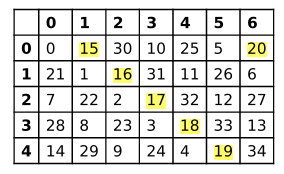
\includegraphics[width=0.5\linewidth]{crt.png}
    \label{fig:enter-label}
\end{figure}

Here we see that if we have a number congruent to 3 modulo 7 and congruent to 1 modulo 5, then it will be congruent to 31 modulo 35.\\\\
We define \(\phi(n) : \mathbb{Z}/m_1m_2\mathbb{Z} \rightarrow \mathbb{Z}/m_1\mathbb{Z} \times \mathbb{Z}/m_2\mathbb{Z}\) as the function that, for a certain \( n \) in the table, gives the modulos in the two other lands.

\newpage

\subsection{RSA}

\subsubsection{Choosing the Parameters}

We choose two large prime numbers \( p \) and \( q \).
We calculate \( m = p \cdot q \), so we can easily calculate \(\Phi(m) = (p-1)(q-1)\).\\\\
The foundation of RSA is that we want \([t^{e \cdot d}]_m = [t]_m\).\\\\
So, \( e \cdot d = \Phi(m) \cdot q + 1 \), and more generally:
\[
e \cdot d + \Phi(m) \cdot k = 1 \quad \text{(1)}
\]
Let's choose a \( p \) and a \( q \rightarrow m = p \cdot q \rightarrow \Phi(m) = (p-1)(q-1)\).\\
Let's choose any \( e \) such that \( \gcd(e, \Phi(m)) = 1 \), see condition (1).\\
Now we need to find a \( d \) that works with our parameters, knowing that we want \( e \cdot d \equiv 1 \pmod{\Phi(m)} \), see condition (1).

\subsubsection{Finding \( d \) Faster}

The problem is that it takes a long time to do this. We can calculate it faster by setting:
\[
k = \mathrm{lcm}(p - 1, q - 1)
\]
This way, we just need to set \( e \cdot d \equiv 1 \pmod{k} \), see condition (1).\\
Why does it work? \(\mathrm{lcm}(p - 1, q-1)\) is a divisor of \((p-1)(q-1) = \Phi(m)\) (it is the smallest number that can be divided by both).\\\\
For example:
\[
10 \cdot 60 = 160 = 2^5 \cdot 5 \quad \mathrm{lcm}(10, 60) = 2^4 \cdot 5
\]
So if \( e \cdot d \equiv 1 \pmod{k} \), it means that 
\[
e \cdot d - 1 = \mathrm{lcm}(p-1, q-1) \cdot q
\]
\[
e \cdot d - 1 = (p-1)(q-1) \cdot q \cdot \text{(missing terms, here 2)}
\]
\[
e \cdot d \equiv 1 \pmod{(p-1)(q-1) = \Phi(m)}
\]
Similarly, the number used for encoding must be coprime with \( k \).\\\\
\(\phi^{-1}(a, b)\), on the contrary, gives us back the two modulos in the original lands.

\newpage

\section{Signature}

We send $t$, the plain text and $[t^d]_m$. $e$ is available to the public. They can compute $[{t^d}^e]_m = [t]_m$ to check whether they get the right plain text again, to see if you are the real sender.\\\\
Because we do not want to send too much data (sending the plaintext twice!), we hash the plaintext with a public function to reduce its size, then compute $[h^d]_m$. The goal for attackers is to seek for a plaintext that would give the same hash.

\section{Channel coding}

bit-rate: $\frac{log_D(M)}{n}$, D is the size of the alphabet, M is the number of codes in the codebook, n is the size of the codes in the codebook

\paragraph{Minimum distance decoding}, we receive a codeword that goes through an error channel, and we pick the code in the codebook with the minimum hamming distance with the errored code.\\\\
Let \( p \) be the maximum weight, the maximum number of errors we can make.

\begin{itemize}
    \item Detection: \( p < d_{\text{min}} \)
    \item Correction: \( p < \frac{d_{\text{min}}}{2} \) (we must stay within the ball of a code)
\end{itemize}

\end{document}
